\documentclass{article}
\usepackage[fleqn]{amsmath}
\usepackage{amssymb,graphicx,color,graphicx,slashed, microtype, parskip, enumitem, extarrows, needspace}
%\usepackage[utf8x]{inputenc}
\usepackage[top=1.5cm, bottom=1.5cm, right=6cm, left=1.5cm, heightrounded, marginparwidth=5cm, marginparsep=0.5cm]{geometry}

\hbadness = 10000
\hfuzz=100pt 
    
\usepackage{marginnote}
\renewcommand*{\marginfont}{\footnotesize}

\usepackage{hyperref}
\hypersetup{colorlinks=true, urlcolor=NavyBlue, bookmarksdepth=3}

\makeatletter\newcommand{\@minipagerestore}{\setlength{\parskip}{\medskipamount}}\makeatother

% =============== Index ===========================

\usepackage[nonewpage]{imakeidx}
\makeindex

% =============== Color Definitions ===============
    
\usepackage[svgnames]{xcolor}
\colorlet{ColorTitle}{Black}
\colorlet{ColorSectionName}{Black}
\colorlet{ColorBoxFG}{Gray}
\colorlet{ColorBoxText}{Black}
\colorlet{ColorBoxBG}{White}


% =============== Title Style ===============
    
\usepackage{titling} % Allows custom title configuration
    
\newcommand{\HorRule}{\color{ColorTitle}\rule{\linewidth}{1pt}} % Defines the gold horizontal rule around the title
    
\pretitle{
    \vspace{-50pt} % Move the entire title section up
    \HorRule\vspace{9pt} % Horizontal rule before the title
    \fontsize{27}{36}\usefont{OT1}{phv}{b}{n}\selectfont
    \color{ColorTitle} % Text colour for the title and author(s)
}
    
\posttitle{\par\vskip 15pt} % Whitespace under the title
    
\preauthor{\fontsize{17}{0}\usefont{OT1}{phv}{m}{n}\selectfont\color{ColorTitle}} % Anything that will appear before \author is printed
    
\postauthor{\par\HorRule}

\newcommand{\COURSENAME}{\href{http://phyw.people.ust.hk/teaching/PHYS2022-2015/}{\textcolor{black}{PHYS 2022}}}
\newcommand{\YW}{\href{http://phyw.people.ust.hk/}{\textcolor{black}{Yi Wang}}}
\newcommand{\PHYS}{\href{http://physics.ust.hk}{\textcolor{black}{Department of Physics}}}
\newcommand{\HKUST}{\href{http://www.ust.hk/}{\textcolor{black}{HKUST}}}
\author{\COURSENAME, \YW, \PHYS, \HKUST}

\date{}

% =============== Section Name Style ===============
    
\usepackage{titlesec}
    
\titleformat{\section}
    {\fontsize{15}{20}\usefont{OT1}{phv}{b}{n}\color{ColorSectionName}}
    {\thesection}{1em}{}
    %[{\vspace{0.2cm}\titlerule[0.8pt]}]
    
\titleformat{\subsection}
    {\fontsize{14}{20}\usefont{OT1}{phv}{m}{n}\color{ColorSectionName}}
    {\thesubsection}{1em}{}
    
\titleformat{\subsubsection}
    {\fontsize{12}{20}\usefont{OT1}{phv}{m}{n}\color{ColorSectionName}}
    {}{0em}{}
      
\setcounter{secnumdepth}{4}
        
% =============== Box Style ===============
    
\usepackage[most]{tcolorbox}
    
\newtcolorbox{tbox}[1]{
    colback=ColorBoxBG, colframe=ColorBoxFG, coltext=ColorBoxText,
    sharp corners, enhanced, breakable, parbox=false,
    before skip=1em, after skip=1em,
    title={#1}, fonttitle=\usefont{OT1}{phv}{b}{n}, 
    attach boxed title to top left={yshift=-0.1mm}, boxed title style={sharp corners, colback=ColorBoxFG, left=0.405cm},
    rightrule=-1pt,toprule=-1pt, bottomrule=-1pt
}

\newtcolorbox{mtbox}[1]{
    colback=ColorBoxBG, colframe=ColorBoxFG, coltext=ColorBoxText,
    sharp corners, enhanced, breakable, parbox=false,
    before skip=1em, after skip=1em,
    title={#1}, fonttitle=\usefont{OT1}{phv}{b}{n},
    attach boxed title to top left={yshift=-0.1mm}, boxed title style={sharp corners, colback=ColorBoxFG, left=0.15cm},
    rightrule=-1pt,toprule=-1pt, bottomrule=-1pt, 
    left=0.5em
}

% =============== tikz has to be loaded after xcolor
\usepackage{tikz}

\newcommand*\enumlabel[1]{\tikz[baseline=(char.base)]{
			\node[shape=rectangle,inner sep=2pt,fill=ColorBoxFG] (char) 
			{\fontsize{7}{20}\usefont{OT1}{phv}{b}{n}{\textcolor{ColorBoxBG}{#1}}};}}

% =============== Useful shortcuts ===============

\newcommand\wref[1]{{\hypersetup{linkcolor=white}\ref{#1}}}  

\newcommand{\textbox}[2]{
    \begin{tbox}{#1}
        #2
    \end{tbox}
}

\newcommand{\mtextbox}[2]{\marginnote{
    \begin{mtbox}{#1}
        #2
    \end{mtbox}}
}

\newcommand{\mnewline}{\vspace{0.5em}\newline}

\newcommand{\titem}[1]{
    \begin{itemize}[label=\color{ColorBoxFG}$\blacktriangleright$, leftmargin=0mm, labelsep=0.27cm, topsep=0.5em
        %, itemsep=1ex
        ]
        #1
    \end{itemize}
}

\newcommand{\mtitem}[1]{
    \begin{itemize}[label={\color{ColorBoxFG}$\blacktriangleright$}, leftmargin=0mm, labelsep=1mm, topsep=0.5em
        %, itemsep=1ex
        ]
        #1
    \end{itemize}
}

\newcommand{\itembox}[3]{
    \begin{tbox}{#1}
        #2
        \titem{#3}
    \end{tbox}
}

\newcommand{\mitembox}[3]{
    \marginnote{
    \begin{mtbox}{#1}
        #2
        \mtitem{#3}
	\end{mtbox}
    }
}

\newcommand{\tenum}[1]{
    \begin{enumerate}[label=\protect\enumlabel{\arabic*}, leftmargin=0mm, labelsep=0.265cm, topsep=0.5em
        %, itemsep=1ex
        ]
        #1
    \end{enumerate}
}

\newcommand{\enumbox}[3]{
    \begin{tbox}{#1}
        #2
        \tenum{#3}
    \end{tbox}
}

\newcommand{\twocol}[5]{
    \begin{minipage}[t][][b]
        {#1\textwidth}
        #4        
    \end{minipage}
    \hspace{#2\textwidth}
    \begin{minipage}[t][][b]
        {#3\textwidth}
        #5
    \end{minipage}
}

\newcommand{\cg}[2]{
    \begin{center}
        \includegraphics[width=#1\textwidth]{#2}
    \end{center}
}

\newcommand{\tbar}{
    ~\newline
    {\color{ColorBoxFG}
    \hbox to 0.15\textwidth{\leaders\hbox to 5pt{\hss  \hss}\hfil} 
    \hbox to 0.7\textwidth{\leaders\hbox to 5pt{\hss . \hss}\hfil}}
    \mnewline
}

% =============== Filter unwanted warnings
\usepackage{silence}
\WarningsOff[tcolorbox]
\hbadness=1000000


\usepackage{bm}
\usepackage{braket}
\graphicspath{{6_fig/}}
\title{第六章\ 量子纠缠和量子信息}

\begin{document}

\maketitle

\textbox{Alice's more adventures in the quantum wonderland}{
    Alice continues to find more about her electron friends:
    \tenum{
        \item \label{item:handstand}
        \marginnote{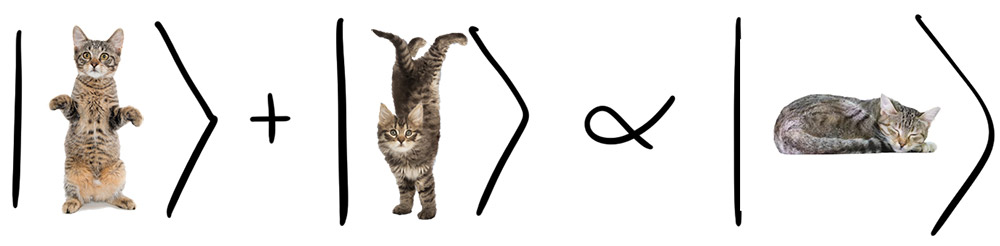
\includegraphics[width=0.35\textwidth]{cat_super_export}\newline Sorry, the above state does not look like an electron. Suppose it is an electron and we will make it clearer later.} 
        superposition of a ``standing'' electron and a ``handstand'' electron is a ``lied-down'' electron. The head direction of the lied-down electron depends on the coefficient of the superposition.
        \item \label{item:information-memory}Alice has very good memory. But she finds it a nightmare trying to remember the relations between a handful of electrons.
        \item \label{item:epr}Alice can show that a measurement of an electron light years away can \emph{immediately} affect the electron state around her. But this superluminal ``quantum information'' does not conflict the causality of special relativity.
        \item \label{item:bell}Alice wants to find out the origin of randomness of the quantum world -- is it due to any hidden local objects that she cannot see? Her electron friends are able to falsify this for her. 
    }
}

\mtextbox{Why use spin for entanglement?}{
    In principle, we would use the familiar position and momentum for entanglement. However, theoretically, continous states are difficult to deal with. Operationally, position eigenstates spread and momentum eigenstates run away. Thus it is much easier (though still extremely difficult) to construct actual devices with spin about quantum entanglement, as the theoretical basis of quantum information and quantum computing.
}
\textbox{Two approaches to the same quantum mechanics}{
    Quantum mechanics can be learned in two ways:
    \tenum{
        \item By first studying the classically most familiar object. The previous Part corresponds to this approach, focusing on the position and momentum of a particle.
        \item By first studying the simplest quantum object. In this part, we will introduce a feature ``spin'' of a quantum particle, with no classical counterpart. 
    }
    \tcblower
    Though these two types of systems appear very different, they follow the same quantum mechanical laws.
}

\section{Spin}\label{sec:spin}

\subsection{The Stern-Gerlach Experiment}

Before stepping into the quantum mechanical world again, let us review a concept which has classical counterpart: the magnetic moment.

\textbox{The magnetic moment\index{magnetic moment}}{
    An object with a magnetic dipole moment (or magnetic moment for short) $\bm{\mu}$ has a magnetic potential energy $U$ when it is put in a magnetic field $\mathbf{B}$\marginnote{Thus, if the magnetic field is inhomogeneous, there is a force acting on the magnetic moment: $\mathbf{F}=-\partial U / \partial \mathbf{r}$.}:
    \begin{align} \label{eq:magnetic-moment}
        U = - \bm{\mu} \cdot \mathbf{B}~.
    \end{align}
    \tcblower
    In our classical world, we are familiar with magnetic moments, and the simplest example is a magnet. A magnetic can be attracted (or repulsed) by another magnetic because of \eqref{eq:magnetic-moment}. Other examples of classical magnetic moment include rotating charges.
}

\textbox{Do atoms have magnetic moment? The Stern-Gerlach experiment\index{Stern-Gerlach experiment}}{
    Let
    \marginnote{\begin{center}
        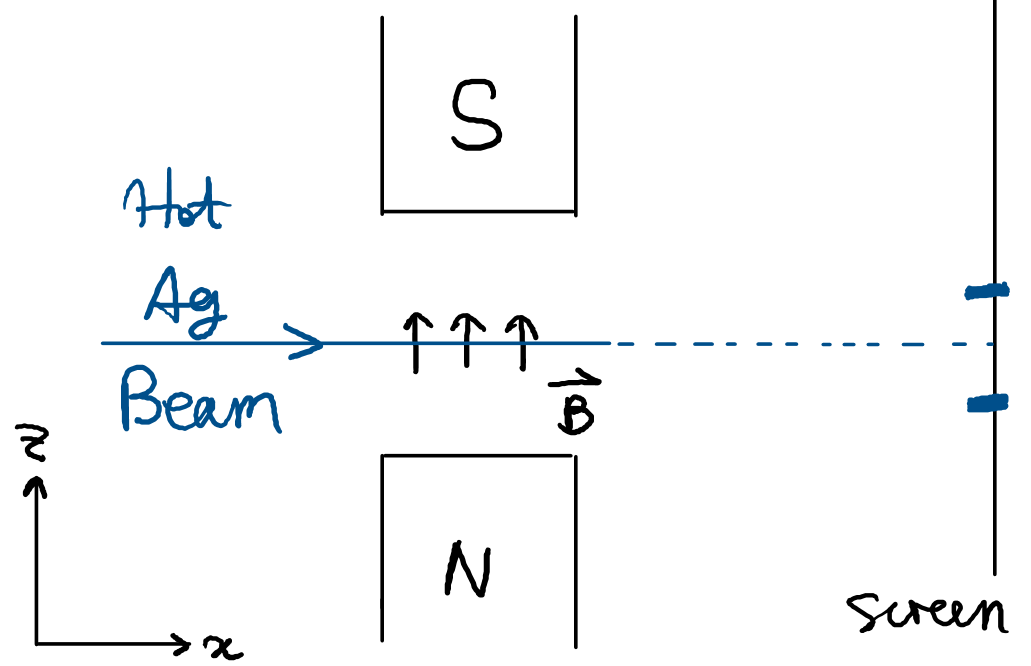
\includegraphics[width=0.35\textwidth]{sgexp}
    \end{center}}
    us now \emph{measure} the magnetic moment of atoms. Consider a beam of hot silver atoms passing through an \emph{inhomogeneous} magnetic field, and the out-going silver atoms leave records on a screen. (The condition ``hot'' indicates that the atoms in the beam have random orientations.)
    
    If we use our \emph{classical} experience to imagine the hot beam of silver atoms. What do we expect? We expect that the result on the screen would be one of the following:
    \tenum{
        \item If silver atoms have no magnetic moment: we still have one beam of silver atoms; the external magnetic field has no effect on the beam.
        \item If silver atoms have nonzero classical magnetic moment: Imagine each silver atom is a magnet with random (and continuously variable) orientation. These magnets experience different forces depending on their orientations, and thus in the limit that there are many magnets, the beam will spread in a continous way. 
    }
    \tcblower
    What is the \emph{actual} outcome of the Stern-Gerlach experiment?

    One beam splits into two beams with equal strength.

    The split of the beam indicates that a silver atom has a magnetic moment $\bm{\mu}$. However, why the split is discrete, instead of continuous?
}

\textbox{The quantum mechanical interpretation of the Stern-Gerlach experiment}{
    We observe two quantum mechanical aspects of the silver atom from the experiment:
    \tenum{
        \item The magnitude $|\bm{\mu}|$ of the silver atom is quantized and cannot vary continuously. 
        \item \label{item:sg-exp-direction}What about the direction $\hat{\bm{\mu}}$? We have two observations:
    }
    \titem{
        \item First, from rotational invariance of the laws of nature, and statistical property of the hot beam, we expect that \emph{before measurement}, i.e. before coming to the external magnetic field, for each silver atom $\bm{\mu}$ should point to random directions.
        \item However, the external magnetic field \emph{measures} the $z$-component of the magnetic moment $\mu_z$ of the atoms, and thus the state of each atom collapses to one of the two eigenstates with eigenvalue $\pm |\bm{\mu}|$, respectively. 
    }
    \tcblower
    These explains the Stern-Gerlach experiment. 
    
    Let us now call the two eigenstates of the magnetic moment in the $z$-direction
    \begin{align}
        \ket{\uparrow} \mbox{ with eigenvalue } |\bm{\mu}| \mbox{, and } \ket{\downarrow} \mbox{ with eigenvalue } - |\bm{\mu}| .
    \end{align}
}

\textbox{The other orientations are superpositions of $\ket{\uparrow}$ and $\ket{\downarrow}$}{
    What about states with other orientations, for example the states pointing inward $\ket{\otimes}$, outward $\ket{\odot}$, left $\ket{\leftarrow}$ and right $\ket{\rightarrow}$?

    As discussed above, after measurement along the $z$-direction, they collapse into states $\ket{\uparrow}$ and $\ket{\downarrow}$. They thus should be superpositions of $\ket{\uparrow}$ and $\ket{\downarrow}$.
    \tcblower
    To further confirm this idea, one can string two Stern-Gerlach experiments in a row: 
    \tenum{
        \item The first magnetic field is in the $y$-direction.
        \item We put another magnet with magnetic field in the $z$-direction before observing the outcome on the screen.
    }
    The outcome of the experiment is: after passing the first magnet, the beams split into two with $\ket{\otimes}$, outward $\ket{\odot}$ states; and each beam further split into $\ket{\uparrow}$ and $\ket{\downarrow}$ after passing the second magnet. Again, the split beams have equal strength.
    
}

\textbox{From atoms to electrons}{
    An electron itself also have magnetic moment. However, if we have used an electron in the Stern-Gerlach experiment, the dominate effect will be the Lorentz force and the magnetic moment is too small to observe. In fact, the magnetic moment of the silver atom comes from the magnetic moment of its outermost (5s) electron, thus indeed shows that the electron has magnetic moment.
}

\mtextbox{Nothing is spinning}{
    The name ``spin'' seems misleading: it provides an intuition that the electron is spinning classically, and thus has a magnetic moment (a spinning charged ball indeed has a magnetic moment classically). 
    \tcblower
    However, for an electron, the spin is a fundamental and instric feature. The electron just has magnetic moment and angular momentum as an instrinic quantum phenomena, because:
    \mtitem{
        \item No experiment shows the electron is actually rotating.
        \item If one uses a rotating ball to explain spin, the rotation speed on the surface of the ball is faster than light, which is not possible.
    }
}
\textbox{Spin and angular momentum\index{spin}}{
    Further experiments show that the magnetic moment of a quantum particle is related to its angular momentum. For an electron,
    \begin{align}
        \mathbf{L} = \frac{1}{2} \frac{m_e}{(-e)} \bm{\mu}~,
    \end{align}
    where $e$ and $m_e$ are charge and mass of an electron, respectively.
    \tcblower
    For historical reasons, the intrinsic magnetic moment of an electron is called ``spin''. In fact, the term ``spin'' is more general than magnetic moment for fundamental particles. Because neutral particles like photons have intrinsic angular momentum as well, but no magnetic moment.
}


\subsection{The Quantum Mechanics of Spins}

In this subsection, we summarize the quantum properties of the spin system. This is a nice application of the quantum mechanics part, and a foundation for studying entanglement.

\textbox{Basis and some other spin states\index{spin states:basis}}{
    In \marginnote{
        For spin, there are only two ``fundamental'' states $\ket{\uparrow}$ and $\ket{\downarrow}$ (basis in the quantum sense). In classical mechanics there are states pointing to all directions, which are all fundamental and cannot be reduced to each other.
        \mnewline
        The other states, say, $\ket{\rightarrow}$, can be written as a linear superposition of $\ket{\uparrow}$ and $\ket{\downarrow}$. In classical mechanics, we can never imagine that up plus down could be equal to right. This explains \ref{item:handstand} in Alice's continued adventures.
    }
    the quantum mechanical language, the indication of equal strength beams in a sequence of Stern-Gerlach experiments is 
    \begin{align}\label{eq:eq-strength-spins}
        \ket{\rightarrow, \leftarrow, \otimes, \odot} =  \frac{1}{\sqrt{2}} \left( \ket{\uparrow} + e^{i\phi}\ket{\downarrow} \right) ~.    
    \end{align}
    The phase turns out to indicate the freedom to choose y and z axes when the x axis is specified. It is convenient to choose:
    \begin{align}
    & \ket{\rightarrow} =  \frac{1}{\sqrt{2}} \left( \ket{\uparrow} + \ket{\downarrow} \right)~, 
    && \ket{\leftarrow} =  \frac{1}{\sqrt{2}} \left( \ket{\uparrow} - \ket{\downarrow} \right)~, \\ 
    & \ket{\otimes} =  \frac{1}{\sqrt{2}} \left( \ket{\uparrow} + i \ket{\downarrow} \right)~, 
    && \ket{\odot} =  \frac{1}{\sqrt{2}} \left( \ket{\uparrow} - i \ket{\downarrow} \right)~.
    \end{align}
}

\textbox{A qubit of information\index{qubit}}{
    A spin state can be thought as the building blocks of information -- a quantum bit (qubit for short) of information. This is because the state has two basis $\ket{\uparrow}$ and $\ket{\downarrow}$. This is to be compared to that a state taking 0 or 1 contains one classical bit of information.

    How much information is contained in a qubit? 
    \marginnote{If we write $\ket{\psi} = \alpha \ket{\uparrow} + \beta \ket{\downarrow}$, we note that normalization of states require $ |\alpha|^2 + |\beta|^2 = 1$, and the overall phase is not relevant. Thus we are left with two real parameters.}

    We need to generalize \eqref{eq:eq-strength-spins}, since in \eqref{eq:eq-strength-spins}, $\ket{\uparrow}$ and $\ket{\downarrow}$ have equal strength. In general this may not be true. Thus, a general state should be 
    \begin{align}
        \ket{\psi} = \cos(\theta/2) \ket{\uparrow} 
        + e^{i\phi} \sin(\theta/2) \ket{\downarrow}~,
    \end{align}
    where $0\leq\theta\leq \pi$, $0\leq \phi<2\pi$. Thus a qubit of information spans a sphere, known as the Bloch sphere.
}

\textbox{Spin states in state vectors\index{spin states: state vectors}}{
    Superpositions and linear operators have the math structure of linear algebra. Thus, one can use vectors to represent spin states, and use matrices to represent operators on them. If we choose $\ket{\uparrow}$ and $\ket{\downarrow}$ as the basis, we can write down the states in the $z$, $x$, $y$ directions as:
    \begin{align} \label{eq:spinmat}
    &\ket{\uparrow} = \begin{pmatrix}1\\0\end{pmatrix}~,
    &&\ket{\downarrow} = \begin{pmatrix}0\\1\end{pmatrix}~,\nonumber \\
    &\ket{\rightarrow} = \frac{1}{\sqrt 2} \begin{pmatrix}1\\1\end{pmatrix}~,
    &&\ket{\leftarrow} = \frac{1}{\sqrt 2} \begin{pmatrix}1\\-1\end{pmatrix}~,\nonumber \\
    &\ket{\otimes} = \frac{1}{\sqrt 2} \begin{pmatrix}1\\i\end{pmatrix}~,
    &&\ket{\odot} = \frac{1}{\sqrt 2} \begin{pmatrix}1\\-i\end{pmatrix}~.
    \end{align}
}

\mtextbox{The analogue for wave functions}{
    Here we are using ``matrix mechanics'' for spins -- find a basis and express things in vectors and matrices. In the Part of Quantum Mechanics, we represent states by wave functions. They are equivalent. For the wave function of the position of a particle, we can write $\psi(x)$ as
    \begin{align*}
        \ket{\psi} = 
        \begin{pmatrix}
            \vdots \\
            \psi(x_1) \\
            \psi(x_2) \\
            \psi(x_3) \\
            \vdots
        \end{pmatrix}~,
    \end{align*}
    Then up to normalization factors, 
    \begin{align*}
        \braket{\psi|\chi} = \int dx ~ \psi^*(x) \chi(x)~.
    \end{align*}
}
\textbox{Inner products of spin states\index{spin states: inner products}}{
    One can define inner products of the state vector. In the matrix sense, if
    \begin{align}
    \ket{\psi} = \begin{pmatrix}a\\b\end{pmatrix}~,
    \qquad
    \ket{\chi} = \begin{pmatrix}c\\d\end{pmatrix}~,
    \end{align}
    define
    \begin{align}
    \bra{\psi} = \begin{pmatrix}a\\b\end{pmatrix}^\dagger
    = (a^*, b^*)~,
    \end{align}
    then
    \begin{align}
    \braket{\psi|\chi} =
     %\begin{pmatrix}a\\b\end{pmatrix}^\dagger 
     (a^*, b^*) \begin{pmatrix}c\\d\end{pmatrix} = a^*c + b^* d~.
    \end{align}
}

\textbox{Normalization and orthogonality of spin states}{
    The normalization conditions of spin states are
    \begin{align}
        \braket{\uparrow|\uparrow} = \braket{\downarrow|\downarrow}
        = \braket{\rightarrow|\rightarrow} = \braket{\leftarrow|\leftarrow}
        = \braket{\otimes|\otimes} = \braket{\odot|\odot} = 1   ~,        
    \end{align}
    And the corresponding pair of states are orthogonal to each other:
    \begin{align}
        \braket{\uparrow|\downarrow}
      = \braket{\rightarrow|\leftarrow}
      = \braket{\otimes|\odot} = 0   ~.
    \end{align} 
    All these conditions can be tested from our construction \eqref{eq:spinmat}.
}

\textbox{Operators for spin measurements in $z$ and $x$, $y$ directions\index{spin states: operators for measurements}}{
    Given the states which have definite spin (spin eigenstates), one can now construct the spin operators, which measures the spin of the state and gives values $\pm 1$.

    One can test that the operators are\marginnote{The trick for a systematic construction is $\sigma_3 = (+1) \times \ket{\uparrow}\bra{\uparrow} + (-1) \times \ket{\downarrow}\bra{\downarrow}$, and similarly for $\sigma_1$ and $\sigma_2$.
    \mnewline
    Here we have defined spin up and down having spin +1 and -1, respectively. In more conventional setup electrons have spins $\pm \hbar/2$. These factors are introduced to compare with the familiar concept of angular momentum. Here we will not include these $\hbar/2$ factors.}
    \begin{align}
    \sigma_3 = \begin{pmatrix}1&0\\0&-1\end{pmatrix}~,
    \quad
    \sigma_1 = \begin{pmatrix}0&1\\1&0\end{pmatrix}~,
    \quad
    \sigma_2 = \begin{pmatrix}0&-i\\i&0\end{pmatrix}~.
    \end{align}
    These operators correspond to the measurements of spin in the $z$, $x$ and $y$ directions, respectively. These operators are known as Pauli matrices.
}

\textbox{Operators for spin measurements in a general direction}{
    From Pauli matrices, it is straightforward to build operators for measurements in a general direction $\hat n$:
    \begin{align}
    \sigma(\hat n) \equiv \sum_i {\hat n}_i \sigma_i = \hat n \cdot \bm{\sigma}~.
    \end{align} 
    \tcblower
    For example, a measurement along 45$^\circ$ direction of the $x$-$z$ plane is
    \begin{align}
    \frac{\sigma_1 + \sigma_3}{\sqrt{2}}  ~.
    \end{align}
}

\textbox{Probability for a measurement to get a particular outcome: $z$ direction}{
    For a spin state $\ket{\psi}$, when measuring the spin of the $z$-direction, the probability to find the spin up state $\ket{\uparrow}$ is \marginnote{To be more precise, in $1+\sigma_3$, the 1 is a shorthand of the identity matrix.}
    \begin{align}
    P_\uparrow = \bra{\psi} \frac{1+\sigma_3}{2} \ket{\psi}~.
    \end{align}
    This is because, the spin state $\ket\psi$ can be in general decomposed into
    \begin{align}
    \ket\psi = \alpha \ket{\uparrow} + \beta \ket{\downarrow}~.
    \end{align}
    Note that\marginnote{Thus $\frac{1+\sigma_3}{2}$ is the projection operator of the spin-up state.}
    \begin{align}
    \frac{1+\sigma_3}{2} \ket{\uparrow} = \ket{\uparrow}~, \frac{1+\sigma_3}{2} \ket{\downarrow}=0~.
    \end{align}
    Thus 
    \begin{align}
    \bra{\psi} \frac{1+\sigma_3}{2} \ket{\psi} = |\alpha|^2~,
    \end{align}
    which is indeed the probability of finding $\ket{\uparrow}$ according to the measurement postulate.
}

\textbox{Probability for a measurement to get a particular outcome: general directions\index{spin states: projection operators}}{
    In general, for the same reason, the probability to find a spin $\ket\psi$ along the $\hat n$ direction after a corresponding measurement is
    \begin{align}
        P_{\hat n} = \bra{\psi} \frac{1+\sigma(\hat n)}{2} \ket{\psi}~.
    \end{align}
}
\mtextbox{Pauli matrices and rotation}{
    In addition to the physical meaning of measurements, there is another physical meaning of Pauli matrices: rotation. The $\sigma_1$, $\sigma_2$, $\sigma_3$ Pauli matrices acting on spin states will rotate the spin along the $x$, $y$, $z$ axis for 180 degrees, respectively. For example, you can understand (up to a phase) how $\sigma_1$, $\sigma_2$, $\sigma_3$ act on $\ket{\uparrow}$ and $\ket{\downarrow}$ using rotation.
    \tcblower
    Why Pauli matrices can mean both measurements and rotations? Mathematically, Pauli matrices are both Hermitian (for measurement) and unitary (for rotation as a transformation).
}
\textbox{Pauli matrices acting on spin states\index{Pauli matrices}}{
    As promised, $\ket{\uparrow}$ and $\ket{\downarrow}$ are eigenstates of $\sigma_3$, such that
    \begin{align}
    \sigma_3 \ket{\uparrow} = \ket{\uparrow}~,
    \quad
    \sigma_3 \ket{\downarrow} = - \ket{\downarrow}~.
    \end{align}
    And it is interesting to note that (as can be tested by direct matrix calculation)
    \begin{align}
    \sigma_1 \ket{\uparrow} = \ket{\downarrow}~,
    \quad
    \sigma_1 \ket{\downarrow} = \ket{\uparrow}~,
    \quad
    \sigma_2 \ket{\uparrow} = i \ket{\downarrow}~,
    \quad
    \sigma_2 \ket{\downarrow} = -i \ket{\uparrow}~.
    \end{align}
}

\section{Multiple Spins and Their Entanglement} \label{sec:entanglement}

\subsection{Multiple Spins, Entanglements, and Quantum Computing}


The last section may not have surprised you since you have already learned some quantum mechanics. However, once we consider two spins, things become surprising again.

\mtextbox{Meaning of states with two arrows}{
    By writing the state $\ket{ab}$ (where $a,b=\uparrow, \downarrow$), we mean just two states $\ket{a}\ket{b}$ considered together. When taking inner products, we take them separately. For example,
    $$
        \braket{cd|ab} = \braket{c|a}\braket{d|b}~,
    $$
    And when we act an operator, we will specify the operator acts on which of the two spin. Mathematically, one can generalize the description with the tensor product of matrices, which is beyond the scope of the present course.
}


Here for simplicity, the two spins are not interacting -- there is no force between them. If we were studying classical mechanics, if two subsystems are not interacting with each other, we can just consider them together for free. Once we know both subsystems, we know the whole system. However, in quantum mechanics, things are different due to the principle of superposition.

\textbox{States with two spins}{
    In a classical world, if we have two spins, each can be in states $\ket{\uparrow}$ and $\ket{\downarrow}$, when considering them together, we get 4 possible states: $\ket{\uparrow\uparrow}, \ket{\uparrow\downarrow}, \ket{\downarrow\uparrow}, \ket{\downarrow\downarrow}$.

    However, in quantum mechanics, superpositions tells that the above 4 states are orthogonal to each other, and thus linear independent. A general state can be written as
    \begin{align}\label{eq:two-qubits}
        \ket{\psi} = \alpha_1 \ket{\uparrow\uparrow} + \alpha_2 \ket{\uparrow\downarrow} + \alpha_3 \ket{\downarrow\uparrow} + \alpha_4 \ket{\downarrow\downarrow}~.
    \end{align}
    \mtextbox{More on quantum information}{
        (Optional) Here we are talking about ``information'' in a sloppy way. The discussion can be made precise with a density matrix
        $$
            \rho = \sum_i p_i \ket{\psi_i}\bra{\psi_i}~,
        $$
        where $p_i$ is the classical probability for the system being in state $i$. 
        Then a whole theory of quantum information can be constructed as a generalization of classical information theory, by considering $\rho$ as a generalization of a list of probabilities. For example, von Neumann entropy $S=-\mathrm{tr} (\rho \ln \rho)$ generalizes the classical Shannon entropy $S = - \sum_i p_i \ln p_i$.
    }
    The state contains two qubits of information.
}
\textbox{Entanglement: How much information is contained in two qubits?\index{entanglement}}{
    We have computed that each qubit is described by $2\times 2 - 2 = 2$ (two complex parameters deducting normalization and overall phase) real parameters. 

    Considering two qubits together, how many real parameters do we need to describe two qubits? 

    Naively, we may expect: each qubit is described by 2 parameters and thus two qubits would be described by 4. Is it correct?

    \tcblower

    In Eq.~\eqref{eq:two-qubits}, there are 4 complex parameters. Deducting normalization and an overall phase, we have $4\times 2 - 2 = 6$ real parameters.

    What are the two unexpected parameters? They describe the entanglement of the two states -- more information when considering the two states together than separately. This is a pure quantum effect and thus hard to imagine or explain classically. You can find the math just in the number counting in this box, and we will discuss some physics about it in the remainder of this section.
}

\needspace{0.2\textheight}
\mtextbox{Realistic quantum computing}{
    Now quantum computers are becoming real. But building a quantum computer challenges the science and technology today. For a quantum computer to work, one needs:
    \mtitem{
        \item Construct the qubits and keep them coherent (maintain the information from quantum entanglement).
        \item Construct quantum gates to operate on qubits.
        \item Design mechanism to correct possible errors from realistic operation.
        \item Design quantum algorithms. See \href{http://math.nist.gov/quantum/zoo/}{Quantum Algorighm Zoo} for currently known quantum algorithms.
    } 
}
\textbox{From $n$ spins to quantum computing\index{quantum computing}\index{quantum information}}{
    How much information is contained in $n$ qubits? We will have $2^n$ basis vectors and thus a general state is described by $2^{n+1} - 2$ real parameters. This explains observation \ref{item:information-memory} of Alice's continued adventures.

    This is exponentially different from classical bits! For $n$ classical bits, the bits can describe \emph{one integer number} with range from $1$ to $2^n$. But $n$ qubits can describe more than $2^n$ numbers. Thus, qubits contain much more information in entanglements -- the information grows exponentially with the number of qubits.
    
    Further, it is possible to manipulate the qubits with ``quantum gates''. For example, the Hadamard gate
    \begin{align}
      \ket{\uparrow} \rightarrow \ket{\rightarrow}~,\qquad \ket{\downarrow} \rightarrow \ket{\leftarrow}
    \end{align}
    and the the ``controlled-NOT'' gate:
    \begin{align}
      \ket{\uparrow\uparrow} \rightarrow \ket{\uparrow\uparrow}~,~~
      \ket{\uparrow\downarrow} \rightarrow \ket{\uparrow\downarrow}~,~~
      \ket{\downarrow\uparrow} \rightarrow \ket{\downarrow\downarrow}~,~~
      \ket{\downarrow\downarrow} \rightarrow \ket{\downarrow\uparrow}~.
    \end{align}

    With quantum information and logical gates to manipulate the information, we get quantum computers!
}

\textbox{Measurements and corresponding operators}{
    For multiple qubits, here we limit our attention to measurements which operates separately on each individual qubit. And for simplicity we consider 2 qubits only.

    The independent measurements can be represented by two set of Pauli matrices, one acting on particle 1 (not affecting particle 2) and the other acting on particle 2 (not affecting particle 1). Let us use $\sigma_i$ to denote the Pauli matrices on particle 1, and use $\tau_i$ to denote the Pauli matrices on particle 2. For example,
\begin{align}
  \sigma_1  \ket{\uparrow\downarrow} = \ket{\downarrow\downarrow} ~, \qquad
  \tau_1  \ket{\downarrow\downarrow} = \ket{\downarrow\uparrow}~.
\end{align}
As $\sigma_i$ and $\tau_i$ act on different spin states, the order of operation $\sigma_i$ and $\tau_i$ commutes. For example, $\sigma_1 \tau_1 \ket{\psi} = \tau_1 \sigma_1 \ket{\psi}$.

As the two measurements are independent, the probability to find particle 1 in direction $\hat n$ and particle 2 in direction $\hat m$ (by measuring corresponding directions) in a state $\ket{\psi}$ is
\begin{align}
  \bra{\psi} \frac{1+\sigma(\hat n)}{2} \frac{1+\tau(\hat m)}{2} \ket{\psi}~. 
\end{align}
}

\subsection{The Einstein-Podolsky-Rosen (EPR) Paradox}

Einstein, though a pioneer of quantum mechanics, has a life-long concern about quantum mechanics. In his philosophy, ``God does not play dice.'' He did not believe that a theory having fundamental randomness would be the complete description of nature. Along this line of thought, in 1935, Einstein, Podolsky and Rosen (EPR) posed the strongest challenge to quantum mechanics. 

\textbox{The EPR state}{
    Let us first prepare a state (known as the ``singlet state'')
\begin{align}
  \ket{s} = \frac{1}{\sqrt{2}} \left ( \ket{\uparrow\downarrow} - \ket{\downarrow\uparrow} \right )~,  
\end{align}
and take the two particles far apart each other. This is possible. For example, a spin-less particle at rest can decay into two particles with opposite spins, and these two particles can fly as far apart as one wants, before they interact with anything else.
}

\textbox{The correlated measurements}{
    Suppose Alice and Bob are light years away from each other. The decay event happens in their middle. Later, Alice receives particle 1 and Bob receives particle 2. They measure the spin of the particles along the $z$-direction immediately after receiving the particles. What will they see?

    We already have the theory to answer this question technically:
    \begin{align}
    & P_{\uparrow\uparrow} = \bra{s} \frac{1+\sigma_3}{2} \frac{1+\tau_3}{2} \ket{s} = 0~, 
    && P_{\downarrow\downarrow} = \bra{s} \frac{1-\sigma_3}{2} \frac{1-\tau_3}{2} \ket{s} = 0~, \nonumber\\
    & P_{\uparrow\downarrow} = \bra{s} \frac{1+\sigma_3}{2} \frac{1-\tau_3}{2} \ket{s} = \frac{1}{2} ~, 
    && P_{\downarrow\uparrow} = \bra{s} \frac{1-\sigma_3}{2} \frac{1+\tau_3}{2} \ket{s} = \frac{1}{2} ~.
    \end{align} 

    In words, both Alice and Bob will find that they have equal chance to find the state having spin up or down. It seems random. But if they meet and compare notes, they will find that their results are totally \emph{correlated} -- if one gets up, the other must get down.

    It is interesting to note that, the above correlation does not depend on the direction that Alice and Bob measure the state. As long as they are measuring the same direction (any $\hat n$), if one gets up, the other must get down. This correlation (without any interactions) is the physical indication of entanglements.
}

\textbox{Does quantum mechanics contradict relativity?\index{EPR paradox}}{
    At
    \marginnote{This explains observation \ref{item:epr} of Alice's continued adventures.}
    first sight, in EPR, information is transmitted faster than light. Thus it contradicts causality in special relativity. This is the EPR paradox.
    \tcblower
    However, there is actually nothing wrong. Before Alice and Bob meet, they consider their own results \emph{random}. Thus Alice cannot encode any information (classical information) in what she choose to measure and let Bob know immediately.  
}

\textbox{Is EPR trivial?}{
    There are many apparent superluminal correlations, which are trivial. For example,
    \tenum{
        \item When a child is born, his/her father immediately becomes a father no matter how far away he is. \label{item:correlation-father}
        \item I pack an apple and an orange into the two boxes. Alice and Bob randomly pick one of them. Then they separate in space. Their measurement about what's in the box will have complete correlation. \label{item:hidden-vars}
    }
    Clearly, these types of correlations cannot send information either. However, is EPR similar to these types of trivial correlations?

    \tcblower

    EPR is not any of them.

    \ref{item:correlation-father} is more trivial. There is correlation, but the correlation is not observable (but rather just a definition) before the father gets any information about the born of the child.

    \ref{item:hidden-vars} is not what happened in EPR, either. In the case of \ref{item:hidden-vars}, Alice and Bob has mutual information,
    \marginnote{
        The mutual information in the apple-orange case is
        $
        I(X;Y) \equiv \sum_{x,y} p(x,y) \log \frac{p(x,y)}{p(x)p(y)} 
         = \log 2
        $. This is just one bit of information in information theory (where the base of log is usually chosen to be 2).
    }
    which is similar to the case of EPR. However, the mutual information is classical information, instead of quantum entanglement.
    
    If Alice choose to measure the spin along the $x$ axis, but Bob still measure long $z$ axis, then their results will not have any correlation (or any further correlations no matter they choose to measure whatever in addition). Whether their results have correlation depends on what they choose to measure. 

    You may not feel satisfied with this explanation -- by measuring different axes, you may argue that one of Alice and Bob destroyed the correlations (recall the collapse of wave function). So this argument is trying to hide (destroy) the difference between EPR and apple-orange instead of trying to compare them honestly. 
    
    Also, 
    \mtextbox{Classical hidden variables}{There are lots of randomness in the classical world due to conditions out of control. For example, when a dice is played, the outcome is (classically) in principle determined by initial condition of the air, perturbations in the air, mechanical property of the desk, etc. But it's too hard to understand these variables to predict the behavior of the dice.\tcblower
    Quantum randomness is fundamentally different, as we will see later.}
    what if we generalize \ref{item:hidden-vars}? The generalization along this line is known as ``local hidden variable theories''. They are theories with hidden variables which are not (yet) observable. 
    
    
    Is it possible to design a better local hidden variable theory (where the randomness of quantum mechanics is due to some variables not-yet-observable), where the ``random'' outcome of EPR (and similarly other quantum measurements) is in fact determined when the two spins were together? And after the states fly apart, each state follow classical logic separately?

    We will show in the next subsection that EPR is indeed intrinsically different from apple-orange in \ref{item:hidden-vars}, and further, no local hidden variable theories can exist.
}

\subsection{The Bell's Inequality and its Violation}

\textbox{Defining a local hidden variable theory in general\index{hidden variable theories}}{
    A local hidden variable theory need to satisfy the follows:
    \tenum{
        \item \emph{Hidden variables}. The apparent quantum behavior follows from some classical logic (where some parts of the system may be hidden so the rest appear random).
        \item \emph{Local}. Space-like measurements do not affect each other.
    }
}

\textbox{A piece of classical logic}{

    Let us prepare many copies of identical EPR pairs. We classify each EPR pair using three classification criteria of states $A$, $B$ and $C$.

    One consequence of the classical logic is: \marginnote{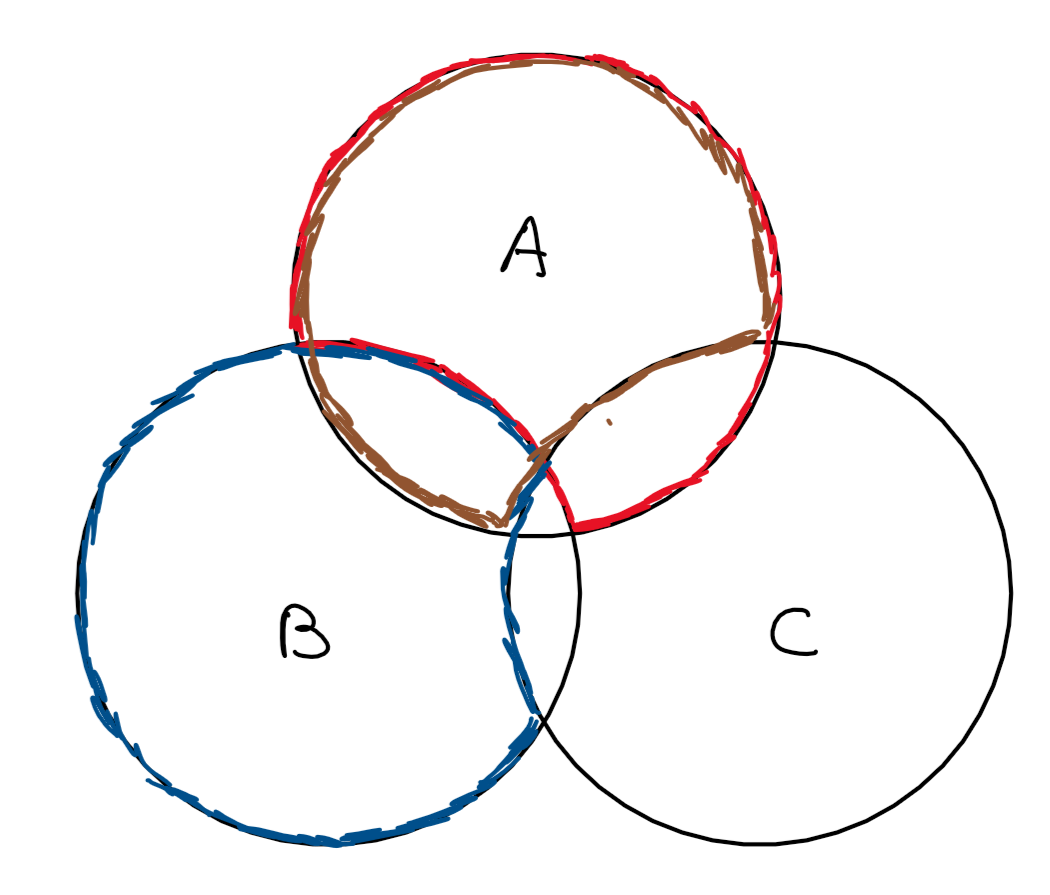
\includegraphics[width=0.4\textwidth]{classical_logic}} 
    \begin{align}\label{eq:classical-logic}
    {\color{red}N(A, \neg B)} + {\color{blue}N(B, \neg C)} \geq {\color{brown}N(A, \neg C)}~,
    \end{align}
    where $N(\cdots)$ denotes the number of states satisfying condition $\cdots$, and $\neg$ denotes ``not''. This relation is illustrated in the figure to the right, where $A$, $B$, $C$ are denoted by circles and the colored contours denote corresponding terms in the above equation.
    \tcblower
    If you consider classical objects and assign, e.g.  $A$: apple (instead of orange); $B$: red (instead of yellow); $C$: sweet (instead of sour). Then \eqref{eq:classical-logic} will always be satisfied. What about EPR pairs with quantum entanglement?
}

\textbox{Testing the classical logic upon the singlet state\index{Bell inequality}}{
    Now let us give meanings of $A$, $B$ and $C$, applying on a singlet state, as measurements by Alice: 

$A$: Measure particle 1 along the $z$-axis and get positive spin.

$B$: Measure particle 1 along $45^\circ$ in $x$-$z$ plane and get positive spin.

$C$: Measure particle 1 along the $x$-axis and get positive spin.

Interestingly, $\neg A$, $\neg B$ and $\neg C$ can be related to measurements by Bob of particle 2 because of the complete anti-correlation:

$\neg A$: Measure particle 2 along the $z$-axis and get positive spin.

$\neg B$: Measure particle 2 along $45^\circ$ in $x$-$z$ plane and get positive spin.

$\neg C$: Measure particle 2 along the $x$-axis and get positive spin.

Eq.~\eqref{eq:classical-logic} with the above conditions is known as the Bell inequality (John Stewart Bell 1964). 

\mtextbox{Why EPR violates Bell inequality?}{
    By violating \eqref{eq:classical-logic}, we are not saying that EPR pairs are not logical. Rather, we cannot assume that each particle in the EPR pair already has features $A$, $B$ and $C$ before the measurement. This is totally different from the apple-orange example.
}


Now it is straightforward to construct probabilities of the events in \eqref{eq:classical-logic}. The probabilities become number of events after a large number of measurements.

\begin{align}
  P(A, \neg B) = \bra{s} \frac{1+\sigma_3}{2} \frac{1+ \frac{\tau_1+\tau_3}{\sqrt{2}}  }{2}   \ket{s} = \frac{1}{4} \left ( 1-\frac{1}{\sqrt 2}  \right )
  \simeq 0.073~. 
\end{align}
\begin{align}
  P(B, \neg C) = \bra{s} \frac{1+ \frac{\sigma_1+\sigma_3}{\sqrt{2}}  }{2} \frac{1+\tau_1}{2}   \ket{s} = \frac{1}{4} \left ( 1-\frac{1}{\sqrt 2}  \right )
  \simeq 0.073~.
\end{align}
\begin{align}
  P(A, \neg C) = \bra{s} \frac{1+ \sigma_3}{2} \frac{1+\tau_1}{2}   \ket{s} = \frac{1}{4} = 0.25~.
\end{align}

Clearly, 
\marginnote{This explains observation \ref{item:bell} of Alice's continued adventures.}
the classical logic \eqref{eq:classical-logic} is violated in this state. Thus the quantum information stored in the entanglement cannot be mimicked by any local hidden variables.
}

\section{Epilogue: Summary and What's Next}

\textbox{Further reading about the content}{
    \titem{
        \item The main reference of this part is Susskind and Friedman, \href{https://www.amazon.com/Quantum-Mechanics-Theoretical-Leonard-Susskind/dp/0465062903}{Quantum Mechanics: The Theoretical Minimum}.
        \item For more information about spin: Sakuri, \href{https://www.amazon.com/Modern-Quantum-Mechanics-Revised-Sakurai/dp/0201539292/ref=sr_1_2?s=books&ie=UTF8&qid=1504076022&sr=1-2&keywords=quantum+mechanics+modern}{Modern Quantum Mechanics}, Chapter 1
        \item For similar content and other Bell-like experiments: Baumann, \href{
            http://www.damtp.cam.ac.uk/user/db275/concepts/Concepts.pdf}{Lecture Notes on Modern Physics}, Chapter 2.
        \item If you'd like to dive deeper in quantum information, read the \href{http://theory.caltech.edu/~preskill/ph229/}{lecture notes by Preskill}.
    }
}

\textbox{What happens next?}{
    Quantum information and quantum computing are fast developing frontiers in research. It is definitely interesting to study them further in quantum mechanics and related courses.
}

\section{Exercises}

\textbox{E\wref{sec:spin}.1 Spin eigenstates}{
    Find the eigenstates and eigenvalues of $\sigma(\hat n)$.
}


\textbox{E\wref{sec:entanglement}.1 Computational details for the Bell inequality}{
    Compute the probabilities $P(A, \neg B)$, $P(B, \neg C)$ and $P(A, \neg C)$.
}

\printindex

\end{document} 